\chapter{Experiments and results}

\section{Ranging system}

\begin{figure}[tbh]
    \centering
    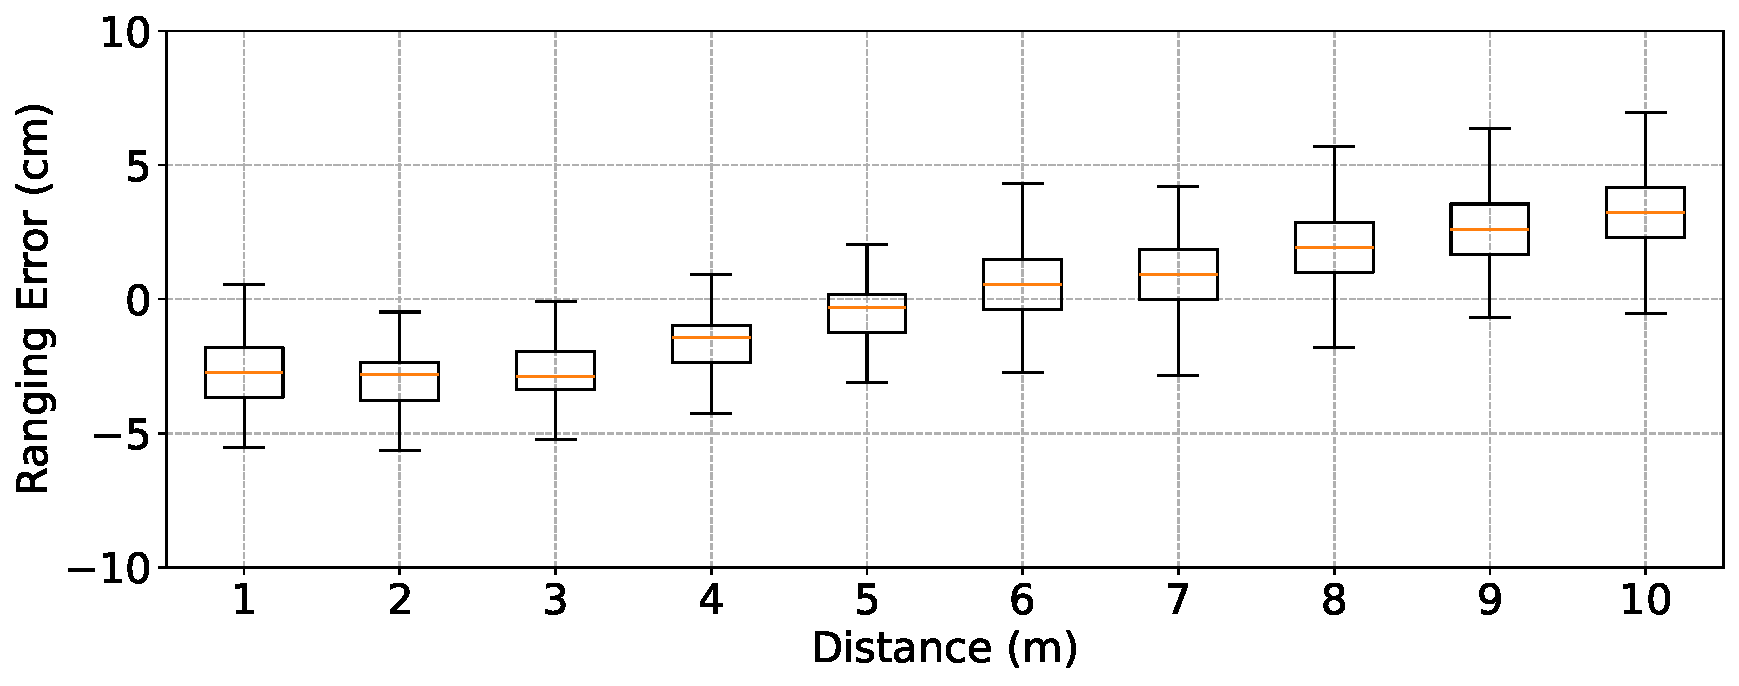
\includegraphics[width=0.8\textwidth]{Figures/experiments_and_results/ranging_accuracy_box.pdf}
    \caption[Distribution of ranging errors.]{Distribution of ranging errors across distances from 1 to 10 meters. Each box represents the interquartile range (IQR), with the horizontal line inside the box indicating the median. Whiskers extend to the data range within 1.5 IQR from the first and third quartiles.}
    \label{fig:ranging_accuracy}
\end{figure}

We evaluate the performance of the proposed ranging system in terms of key operational metrics, namely: (i) ranging accuracy and precision, (ii) ranging frequency, and (iii) quality of TDMA-based synchronization for multi-anchor operation. 

A single anchor and a fixed tag were used to collect ranging measurements at distances from 1 to 10 meters to assess the accuracy of the ranging system. At each location, \SI{\approx 1000}{} range estimates were recorded under LoS conditions. The resulting errors between measured and ground-truth distances are summarized in \autoref{fig:ranging_accuracy}. As expected, a slight systematic bias is observed: distances are underestimated at short range and overestimated at long range. This behavior is attributed to the threshold-based ToF estimation algorithm, discussed in \autoref{lde}, wherein signals with higher amplitude exhibit steeper rising edges and thus cross the detection threshold earlier than weaker signals with slower rise times.  Despite this, the absolute median error remains within \SI{\pm 5}{\centi\metre} bounds across all distances, with the overall dispersion of \SI{\approx 3}{\centi\metre}, indicating high precision.

\begin{figure}[tbh]
    \centering
    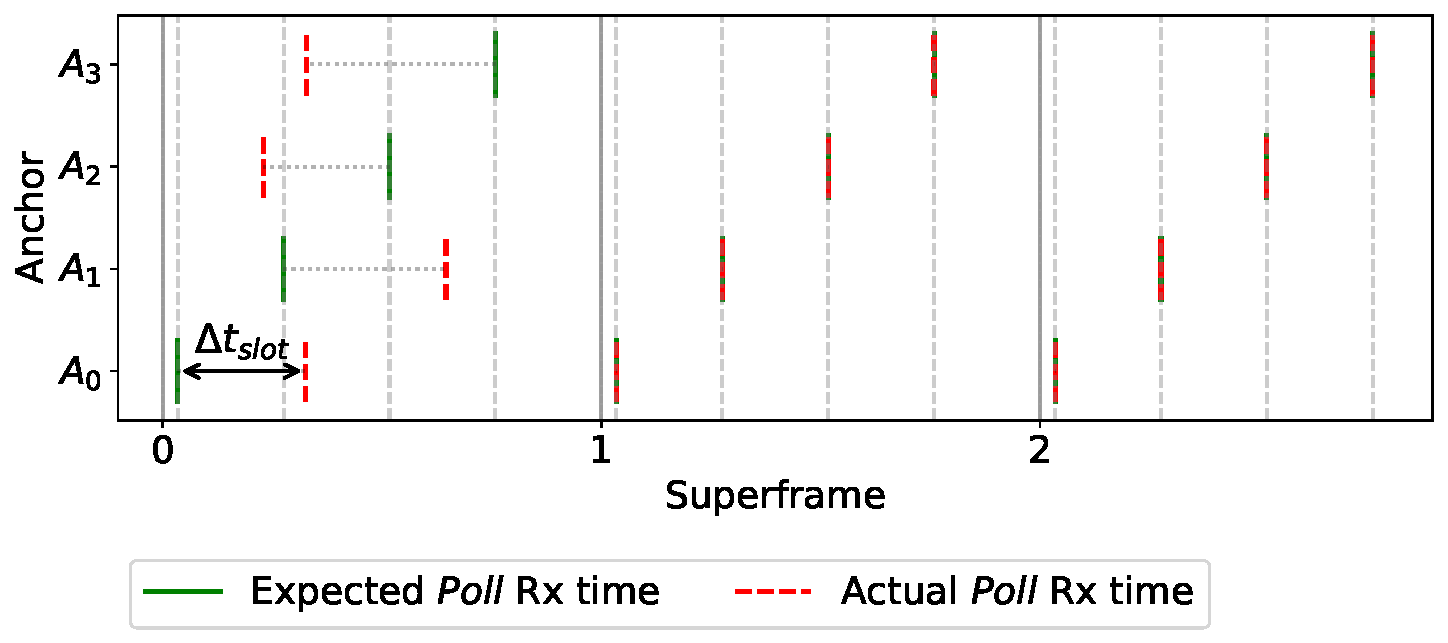
\includegraphics[width=0.8\textwidth]{Figures/experiments_and_results/sync_visualize.pdf}
    \caption[Slot synchronization timeline for a four-anchor deployment.]{Slot synchronization timeline for a four-anchor deployment. Green lines indicate the expected reception times of \textit{Poll} messages at the tag, while red dashed lines denote the actual reception times.}
    \label{fig:sync}
\end{figure}

To assess the quality of inter-device synchronization (refer to \autoref{ranging_system} for details), the timing alignment of received \textit{Poll} messages was evaluated over consecutive superframes when four anchors are active. As stated before, the observed offset, $\Delta t_{\text{slot}}$, is continuously estimated at the tag and relayed back to the anchor, which then adjusts its future slot scheduling. \autoref{fig:sync} visualizes this process. Initially, noticeable misalignments between expected and actual message arrival times are observed. However, convergence is achieved within two superframes. After correction, the residual timing jitter remains as low as approximately \SI{1}{\micro\second}.

In the current configuration, each slot was assigned a duration of \SI{3700}{\micro\second}, with a guard interval of \SI{500}{\micro\second} added at the beginning of each superframe to accommodate wake-up uncertainty and prevent overlap. This scheduling yields an effective measurement frequency of approximately \SI{67}{\hertz} per anchor, resulting in a combined rate of \SI{270}{\hertz} for the four-anchor setup used in the experiments.

\section{Dataset analysis}

\begin{figure}[tbh]
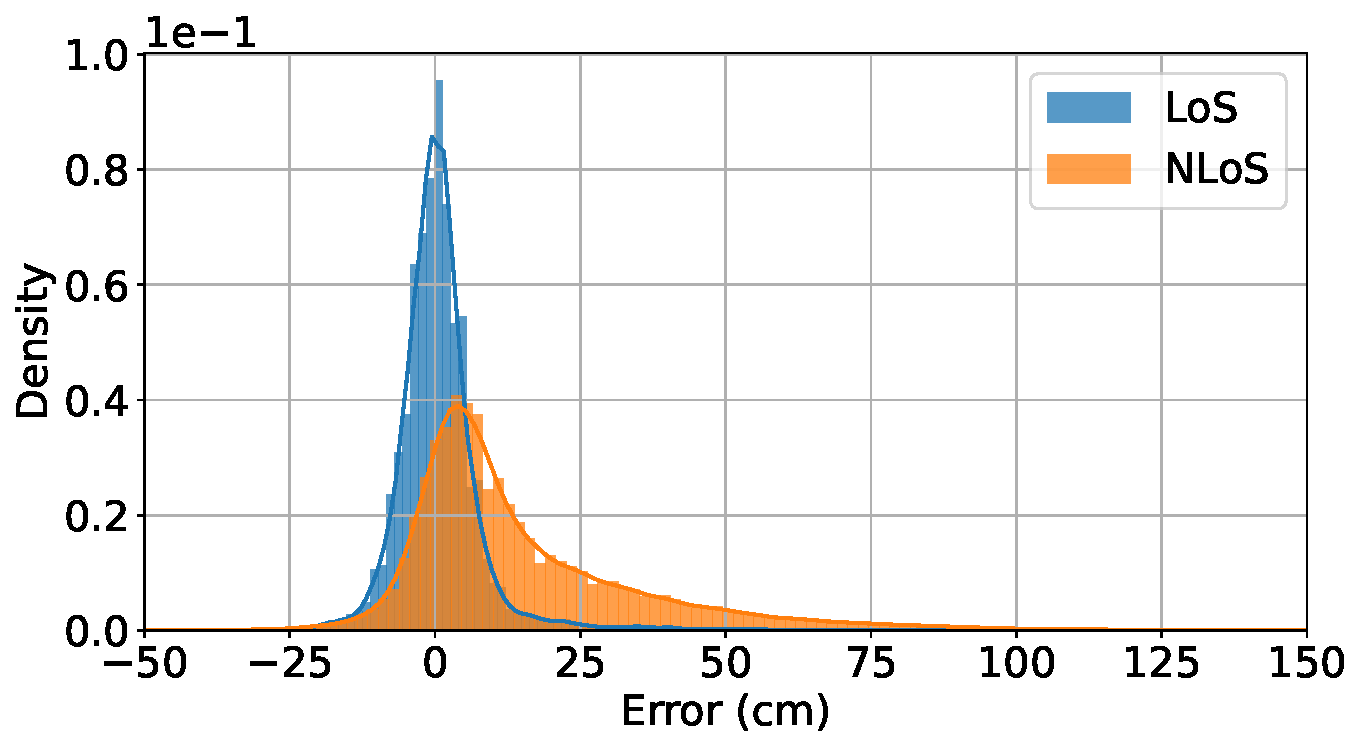
\includegraphics[width=0.7\textwidth]{Figures/experiments_and_results/dataset_error_distribution.pdf}
\centering
\caption[Empirical distribution of ranging errors in \textit{RangeCIR} dataset.]{Empirical distribution of ranging errors in \textit{RangeCIR} dataset under LoS and NLoS conditions.}
\label{fig:err_dist}
\end{figure}

The \textit{RangeCIR} dataset presented in \autoref{data_collection} consists of 990\,147 samples, spanning ranges between 1 and 7.5 meters. The experimental procedure ensured comprehensive coverage of both LoS and realistic NLoS scenarios, simulated with human obstruction, yielding a balanced distribution of approximately \SI{55}{\percent} LoS and \SI{45}{\percent} NLoS samples. \autoref{fig:err_dist} illustrates the empirical distribution of ranging errors under LoS and NLoS conditions. The LoS errors exhibits a sharp unimodal peak centered around zero, indicative of stable and low-variance performance under unobstructed conditions. Conversely, the NLoS error distribution is positively skewed with increased dispersion, closely resembling a log-normal distribution for the positive-valued portion of the data, reflecting multipath-induced bias due to human obstructions.

\begin{table}[tbh] 
\centering 
\caption[Summary of ranging error statistics in the proposed dataset.]{Summary of ranging error statistics in the proposed dataset. $\mu$: mean error, $\sigma$: standard deviation, MAE: mean absolute error. All values in centimeters.} \label{tab:error_stats} 
\begin{tabular}{lccc} 
\toprule 
\textbf{Condition} & $\mathbf{\mu}$ & $\mathbf{\sigma}$ & \text{MAE} \\ 
\midrule 
LoS & 3.6 & 7.7 & 5.6 \\
NLoS & 18.4 & 21 & 19.4 \\
Overall & 10.3 & 16.9 & 11.8 \\ 
\bottomrule 
\end{tabular} 
\end{table}

\autoref{tab:error_stats} summarizes the statistical properties of these errors. Across the entire dataset, the ranging error varies from \SI{-50}{\centi\metre} to \SI{219}{\centi\metre}, yielding a mean of \SI{10.3}{\centi\metre}, a standard deviation of \SI{16.9}{\centi\metre}, and a mean absolute error (MAE) of \SI{11.8}{\centi\metre}. For isolated LoS measurements, we report a mean of \SI{3.6}{\centi\metre}, and a standard deviation of \SI{7.7}{\centi\metre}. In contrast, the data labeled as NLoS has significantly higher bias and dispersion (mean \SI{18.4}{\centi\metre}, standard deviation \SI{21}{\centi\metre}), resulting in an MAE of \SI{5.6}{\centi\metre} for LoS and \SI{19.4}{\centi\metre} for NLoS measurements.


\section{A-REMNet results}

\subsection{Training and inference setup}
The proposed A-REMNet model was implemented in PyTorch Python framework and trained on a filtered subset of the collected dataset (\autoref{data_collection}). To prevent overfitting to LoS conditions, which tend to exhibit low error variability, the dataset was rebalanced to contain \SI{70}{\percent} NLoS samples. The resulting dataset comprised 640\,715 samples, partitioned into training, validation, and test subsets (70/20/10), with measurement samples randomly distributed across splits.

CIR samples were extracted as complex-valued tensors of shape $K \times 2$, where $K = 133$ corresponds to a fixed window around the first path index, including 5 samples before and 127 after. This window was empirically selected for optimal performance. Each CIR sample was paired with a scalar ground truth error label.

Model hyperparameters were tuned using Bayesian optimization on the validation set. The final configuration included $F = 64$ low-level feature channels and $N = 5$ RRMs. To balance complexity and ensure sufficient temporal resolution for effective operation, a self-attention unit with $h = 4$ heads was included in the first two RRMs only. The reduction ratio of the SE block is set to $r = 8$. The kernel sizes of the convolutional layers are retained from the original study: 7 for the initial convolution, 3 for the residual units and the first branch of the reduction block, and 1 for the second branch. This configuration results in approximately 200K trainable parameters.

To assess computational feasibility, empirical complexity analysis was conducted using Meta's \texttt{fvcore} profiling tool. The model was found to require approximately 11.7 million floating-point operations (FLOPs) per forward pass. Inference latency was measured on an NVIDIA GeForce RTX 2080Ti GPU, yielding a mean runtime of \SI{2.9}{\milli\second} per sample with a standard deviation of \SI{0.05}{\milli\second}.

Training was performed with a batch size of 256 for up to 100 epochs using the Adam optimizer with a learning rate of $10^{-3}$. To prevent overfitting, early stopping with a patience of 5 epochs was applied based on validation loss monitoring. To handle the heavy-tailed error distribution of the dataset, particularly under NLoS conditions, the model was trained using the Huber loss, which balances sensitivity to small errors with robustness to outliers:

\begin{equation} 
\mathcal{L}_{\delta}(e) = 
\begin{cases} 
\frac{1}{2}e^2, & \text{if}\ |e| \leq \delta,\\
\delta \left(|e| - \frac{1}{2}\delta\right), & \text{otherwise}, 
\end{cases} 
\end{equation}
where $e$ denotes the prediction error and $\delta = 1.0$ defines the transition point between quadratic and linear regimes. The training process is completed in approximately 20 minutes.

\subsection{Quantitative results}

\begin{table}[tbh] 
\centering 
\caption[Error statistics before and after mitigation.]{Error statistics on the test set before and after mitigation. All values in centimeters. Refer to \autoref{tab:error_stats} for notation definitions.} 
\label{tab:test_results} 
\begin{tabular}{lccc|ccc|c} 
\toprule 
\multirow{2}{*}{\textbf{Condition}} 
& \multicolumn{3}{c|}{\textit{Before mitigation}} 
& \multicolumn{3}{c|}{\textit{After mitigation}} 
& \textit{Improvement} \\
& $\mu$ & $\sigma$ & MAE & $\mu$ & $\sigma$ & MAE & $\Delta$MAE \\
\midrule 
LoS     & 3.7  & 7.8  & 5.6  & -0.2 & 3.8 & 2.2 & \textbf{61 \%} \\
NLoS    & 18.3 & 21.1 & 19.4 & 0.8  & 9.8 & 5.5 & \textbf{71 \%} \\
Overall & 14.0 & 19.4 & 15.3 & 0.5  & 8.5 & 4.5 & \textbf{70 \%} \\
\bottomrule 
\end{tabular} 
\end{table}

\autoref{tab:test_results} reports error statistics on the test set. The model reduces the overall MAE from \SI{15.3}{\centi\metre} to \SI{4.5}{\centi\metre}, corresponding to a relative improvement of \SI{70}{\percent}. Notably, even in LoS conditions, where errors are typically low, the model still reduces the MAE from \SI{5.6}{\centi\metre} to \SI{2.2}{\centi\metre}, amounting to a \SI{61}{\percent} relative improvement. This suggests that the network learned to model subtle, deterministic biases present in LoS CIRs, which we believe likely arise from antenna orientation characteristics. In NLoS scenarios, where the error variance is higher, the MAE decreases from \SI{19.4}{\centi\metre} to \SI{5.5}{\centi\metre}, yielding a relative improvement of \SI{71}{\percent}. In all cases, the standard deviation of residuals is also significantly lower, indicating improved consistency across estimates.

\begin{figure}[tbh] 
\centering 
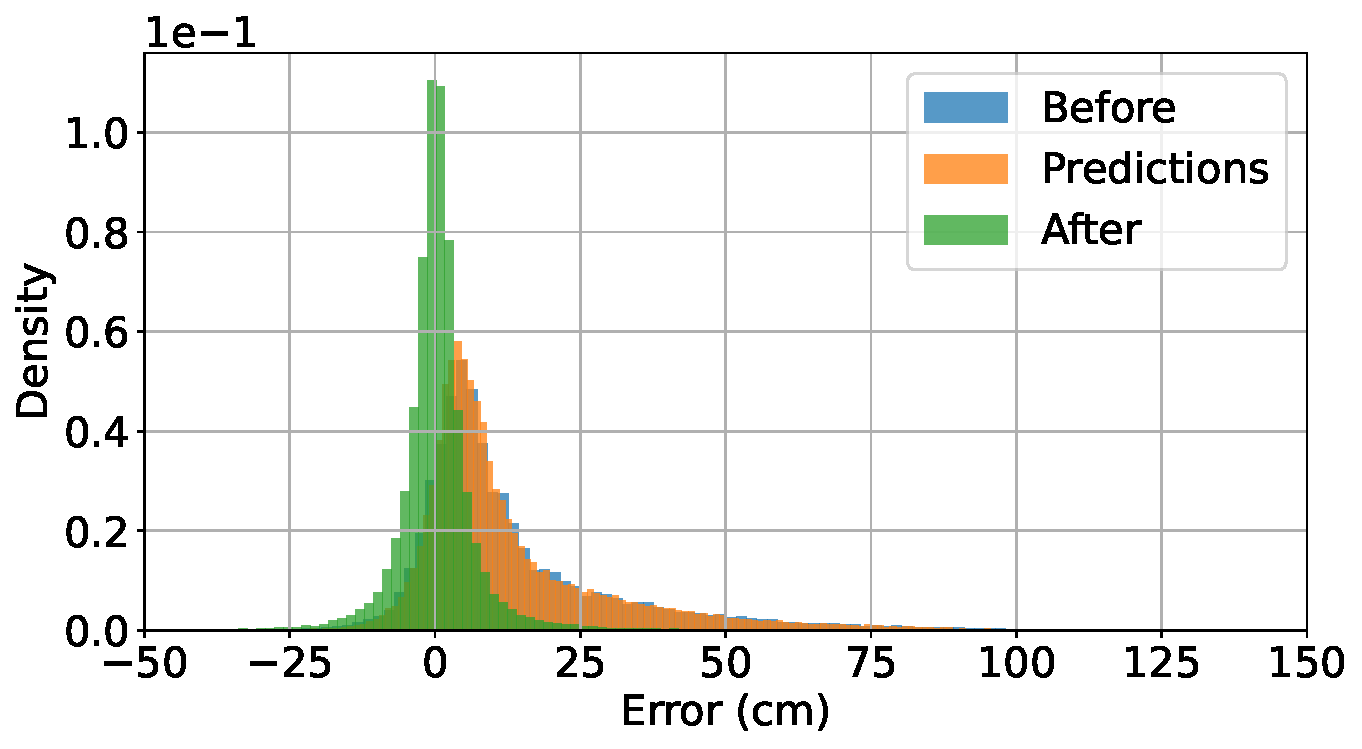
\includegraphics[width=0.7\textwidth]{Figures/experiments_and_results/model_error_distribution.pdf} 
\caption[Distributions of errors before and after mitigation.]{Distributions of errors before and after mitigation, along with model-predicted errors on the test set.} \label{fig:error_distribution} 
\end{figure}

\autoref{fig:error_distribution} shows the empirical distributions of observed, predicted, and residual errors. Notably, the residual error distribution is approximately Gaussian, centered near zero ($\mu = 0.5$). This is a desirable property in localization pipelines, where zero-mean noise aligns with common assumptions in Kalman filters (\autoref{kalman_theory}).

\subsubsection{Ablation study}
To assess the contribution of the proposed attention mechanism, we conducted an ablation study by removing the attention unit from each RRM, while preserving all other architectural components, hyperparameters, training configuration, and dataset splits. The resulting baseline model is structurally identical to A-REMNet, apart from the absence of the attention unit, and comprises 151\,337 trainable parameters (compared to 200\,425 in the full model).

\begin{table}[tbh]
\centering
\caption[Error statistics with and without the attention mechanism.]{Comparison of test set error statistics with and without the attention mechanism. All values in centimeters. Refer to \autoref{tab:error_stats} for notation definitions.}
\label{tab:ablation_results}
\begin{tabular}{lccc|ccc|c}
\toprule
\multirow{2}{*}{\textbf{Condition}} &
\multicolumn{3}{c|}{\textit{No Attention}} &
\multicolumn{3}{c|}{\textit{With Attention}} &
\textit{Improvement} \\
& $\mu$ & $\sigma$ & MAE & $\mu$ & $\sigma$ & MAE & $\Delta$MAE \\
\midrule
LoS     & -0.7 & 4.1  & 2.4 & -0.2 & 3.8 & 2.2 & \textbf{8 \%} \\
NLoS    & 1.0  & 11.0 & 6.3 & 0.8  & 9.8 & 5.5 & \textbf{13 \%} \\
Overall & 0.5  & 9.5  & 5.1 & 0.5  & 8.5 & 4.5 & \textbf{12 \%} \\
\bottomrule
\end{tabular}
\end{table}

\autoref{tab:ablation_results} summarizes the results for both variants. Removal of the attention unit results in a degradation of error mitigation performance across all conditions. The overall MAE increases from \SI{4.5}{\centi\metre} to \SI{5.1}{\centi\metre}, corresponding to a relative improvement of \SI{12}{\percent} in favor of the attention-based model. This is accompanied by a higher standard deviation of residuals (\SI{9.5}{\centi\metre} vs.\ \SI{8.5}{\centi\metre}). The effect is most pronounced under NLoS conditions, where the residual MAE increases by \SI{13}{\percent}, from \SI{5.5}{\centi\metre} to \SI{6.3}{\centi\metre}. Interestingly, however, a performance gap of \SI{8}{\percent} is also observed under LoS conditions, where MAE increases from \SI{2.2}{\centi\metre} to \SI{2.4}{\centi\metre}, indicating that the attention unit is beneficial even in lower-error conditions.

These results suggest that the self-attention mechanism contributes substantially to the model's ability to extract temporal dependencies in the CIR sequence and suppress likely complex error patterns, particularly under NLoS conditions.


\section{Experimental results}

To evaluate the end-to-end performance of the proposed IPS pipeline, which integrates A-REMNet-based error mitigation with EKF-based localization, we conducted a series of trajectory reconstruction experiments under varying conditions. Three scenarios were tested: (i) no obstacles (clear LoS), (ii) obstructed paths in a known (seen before) environment used during dataset collection (see \autoref{data_collection}), and (iii) obstructed paths in a previously unseen environment. Each scenario included two movement patterns: a rectangular loop and an hourglass-shaped trajectory.

\subsection{Experimental setup}

\begin{figure}[tbh]
    \centering
    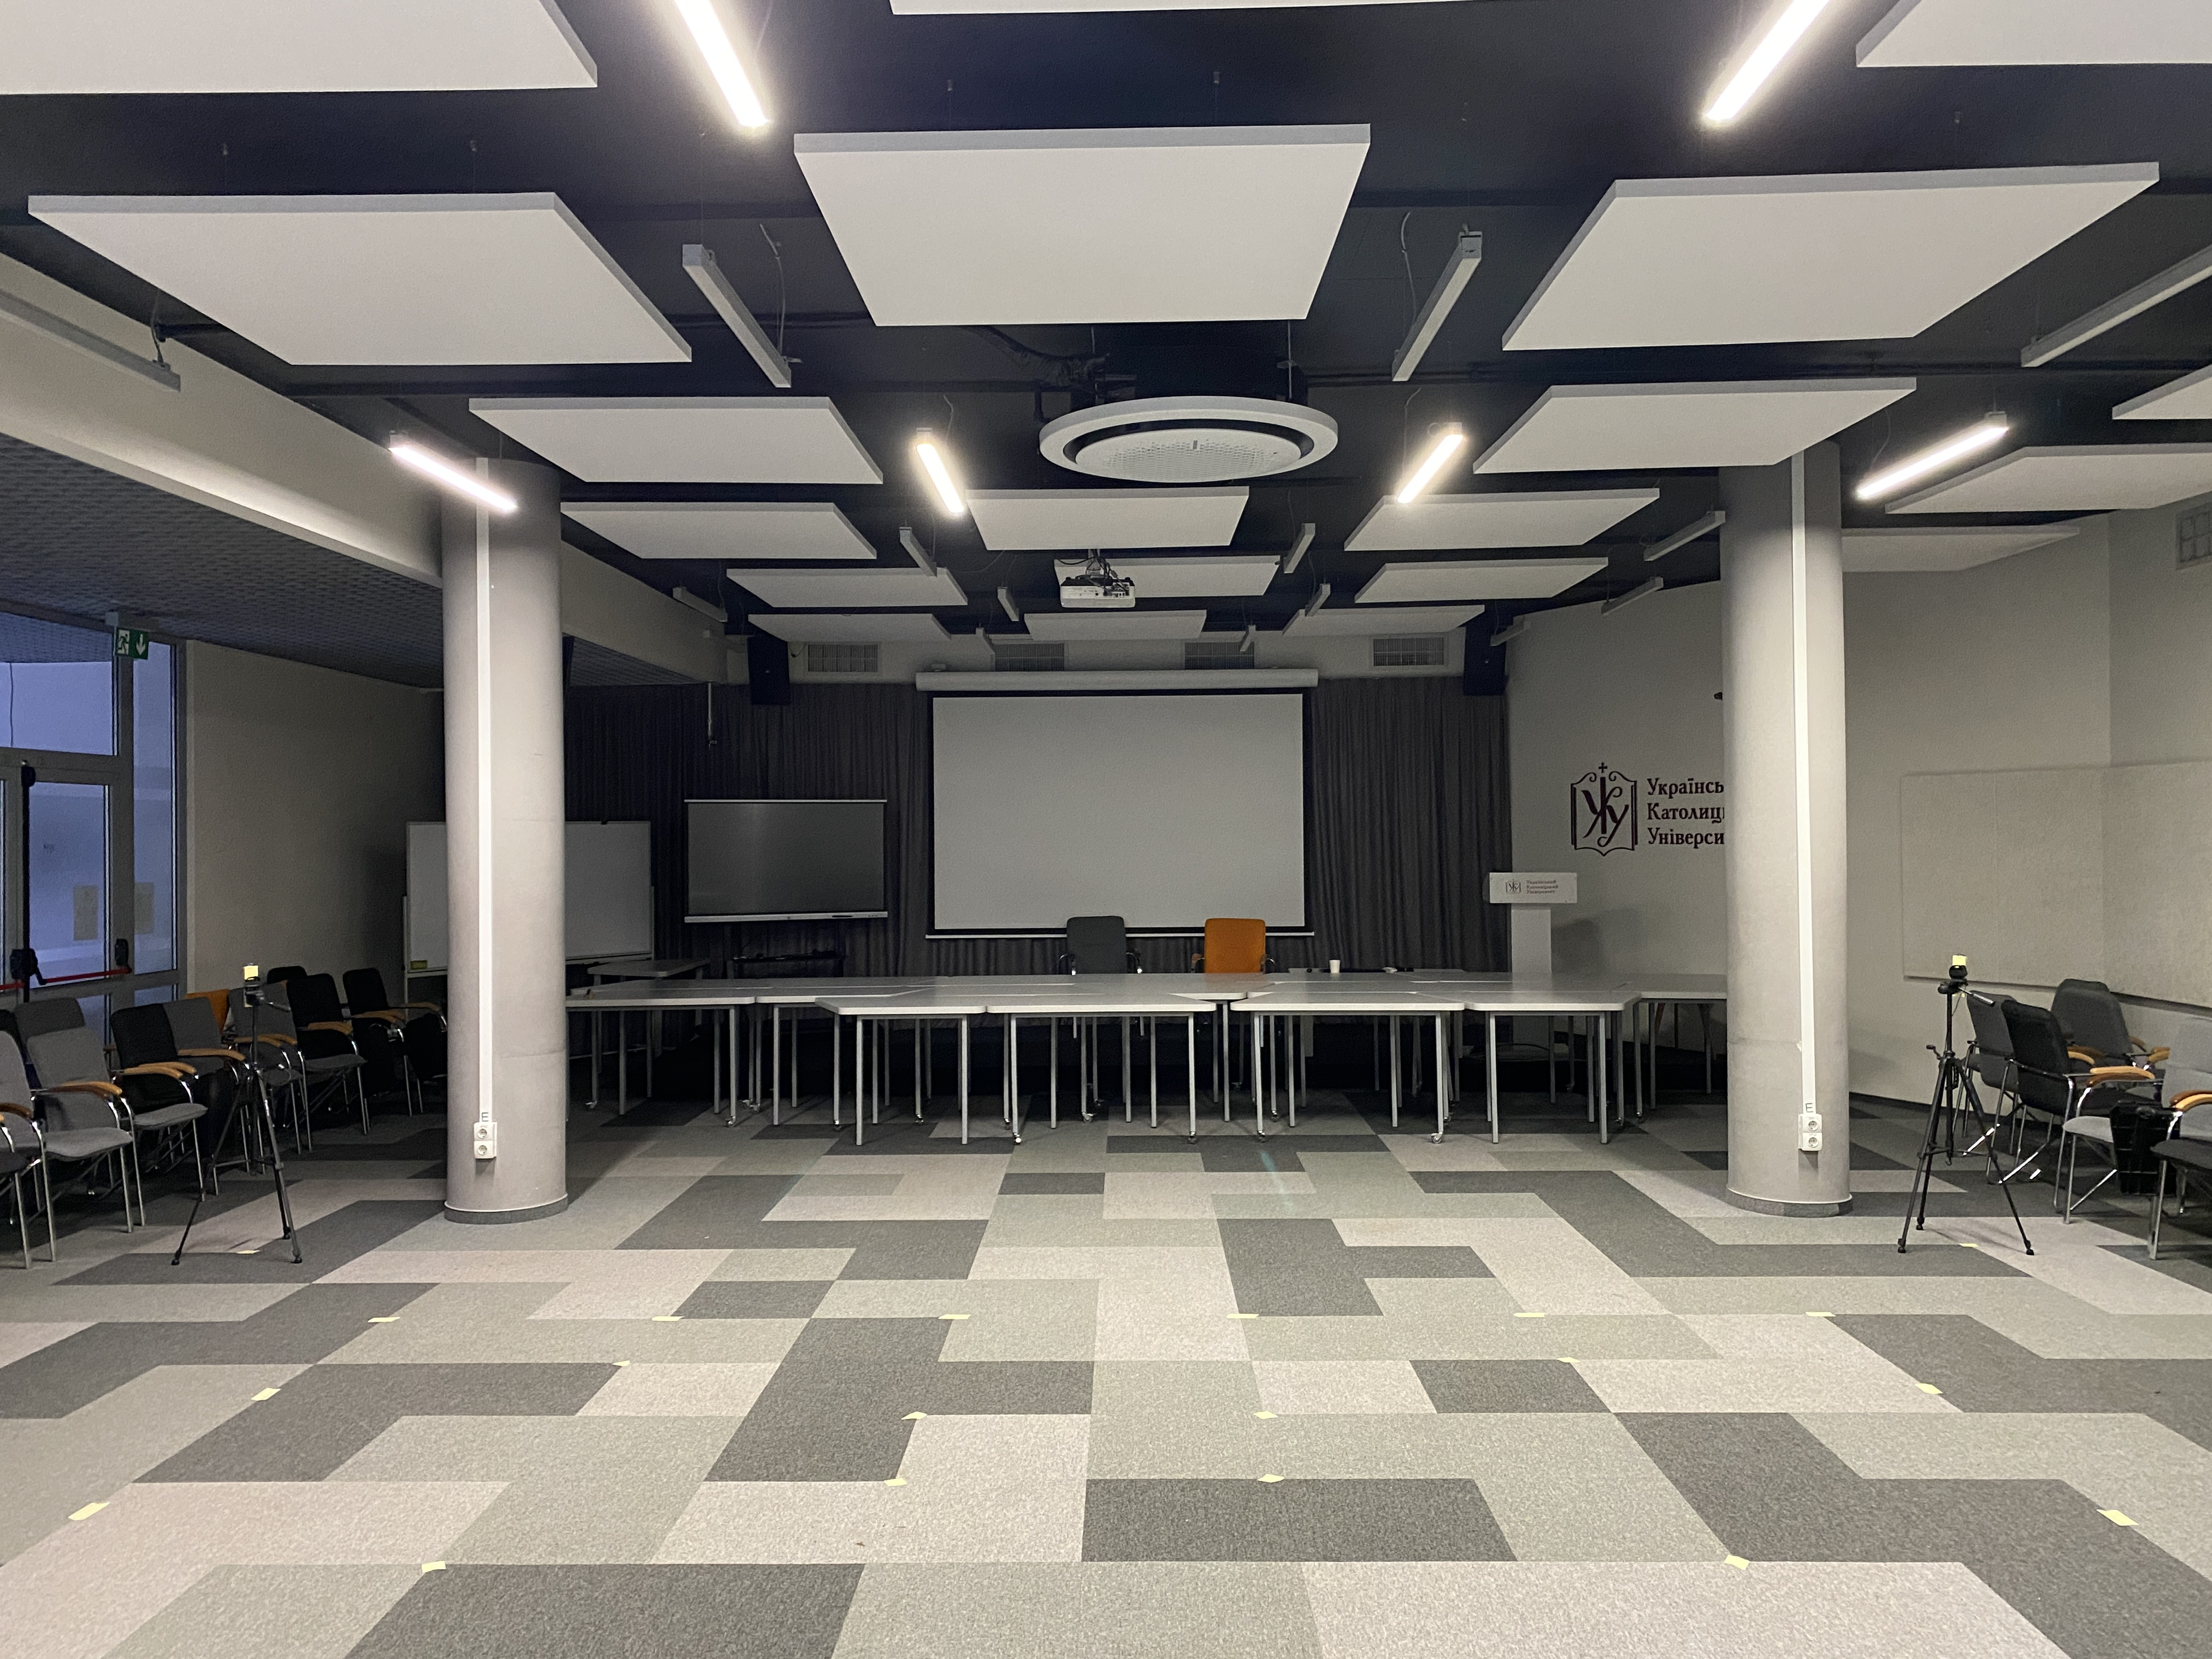
\includegraphics[width=0.7\textwidth]{Figures/experiments_and_results/evaluation_env.png}
    \caption[Unseen evaluation environment.]{Unseen evaluation environment. The space differs structurally, geometrically, and visually from the training environment.}
    \label{fig:unseen_environment}
\end{figure}

All experiments were carried out in indoor environments, with four UWB anchors mounted on tripods around the corners of the trajectory frame. The tag was handheld and moved by a human subject at a consistent walking speed (\SI[per-mode=symbol]{\approx 3}{\kilo\metre\per\hour}) along pre-marked paths. For the obstructed configurations, four individuals continuously moved along the LoS paths between the transceivers, thereby maintaining persistent blockage of the direct signal path. We want to elaborate, that the unseen environment, depicted in \autoref{fig:unseen_environment}, was not used during training, and serving as a testbed for evaluating the generalization capability of the error mitigation model.

Ground truth positions were derived from the known trajectory geometry, with synchronization timing recovered from ceiling-mounted camera video recordings. Due to inherent human movement variance, the subject's adherence to the marked trajectory was accurate to within approximately \SI{10}{\centi\meter}. Given the slight remaining mismatch in timing between the human-executed path and the inferred ground-truth position estimates, particularly around corners, the Dynamic Time Warping (DTW) algorithm~\cite{dtw}, implemented via the \texttt{fastdtw} Python library, was used to temporally align the estimated and reference trajectories by computing an optimal index-wise correspondence between them under continuity and monotonicity constraints. The resulting warping path was used to derive pointwise errors and enabled robust MAE evaluation, despite natural speed variations.

% Given the slight remaining mismatch in timing between the human-executed path and the inferred ground-truth position estimates, especially around trajectory corners, the DTW algorithm~\cite{dtw} was applied to align the estimated and ground-truth trajectories. 

% Let $\mathbf{X} = \{ \mathbf{x}_1, \dots, \mathbf{x}_N \}$ and $\mathbf{Y} = \{ \mathbf{y}_1, \dots, \mathbf{y}_M \}$ denote the estimated and ground truth trajectories, respectively. DTW computes an optimal alignment path $\mathcal{W}$ of length $K$, defined as a sequence of index pairs $(i_k, j_k) \mid i_k \in [1, N],\ j_k \in [1, M]$, by minimizing the total pointwise Euclidean distance under continuity and monotonicity constraints:
% \begin{equation}
% \mathcal{W}^* = \arg \min_{\mathcal{W}} \sum_{k=1}^{K} \| \mathbf{x}_{i_k} - \mathbf{y}_{j_k} \|_2.
% \end{equation}
% Each pair $(i_k, j_k)$ indicates that the $i_k$-th point of the estimated trajectory is matched with the $j_k$-th point of the ground truth trajectory. The resulting path was used to derive pointwise absolute errors, enabling robust computation of the MAE even in the presence of natural speed variations.


Under conditions without obstacles, we conducted only three repetitions of each experiment due to low variance in the resulting measurements. For setups with obstacles, each experiment was repeated five to seven times to ensure statistical significance of the results. For each experiment, the estimated range measurements were processed through the proposed Kalman filter, applied in two variants: with and without prior error correction using A-REMNet model. The filter parameters were tuned using the normalized innovation squared (NIS) and normalized estimation error squared (NEES) metrics to ensure the statistical consistency of the filter. Specifically, we select noise covariances $\mathbf{Q}, \mathbf{R}$ such that \SI{\approx 95}{\percent} of the NIS and NEES values remained within the theoretical confidence bounds ($\chi^2$ distribution) for their respective degrees of freedom. In our experiments, we set $\mathbf{Q} = 10^{-4} \cdot \mathbf{I}_4$, and $\mathbf{R} = 0.3$.

\subsection{Performance evaluation}
\subsubsection{Quantitative results}

\begin{figure}[tbh]
    \centering
    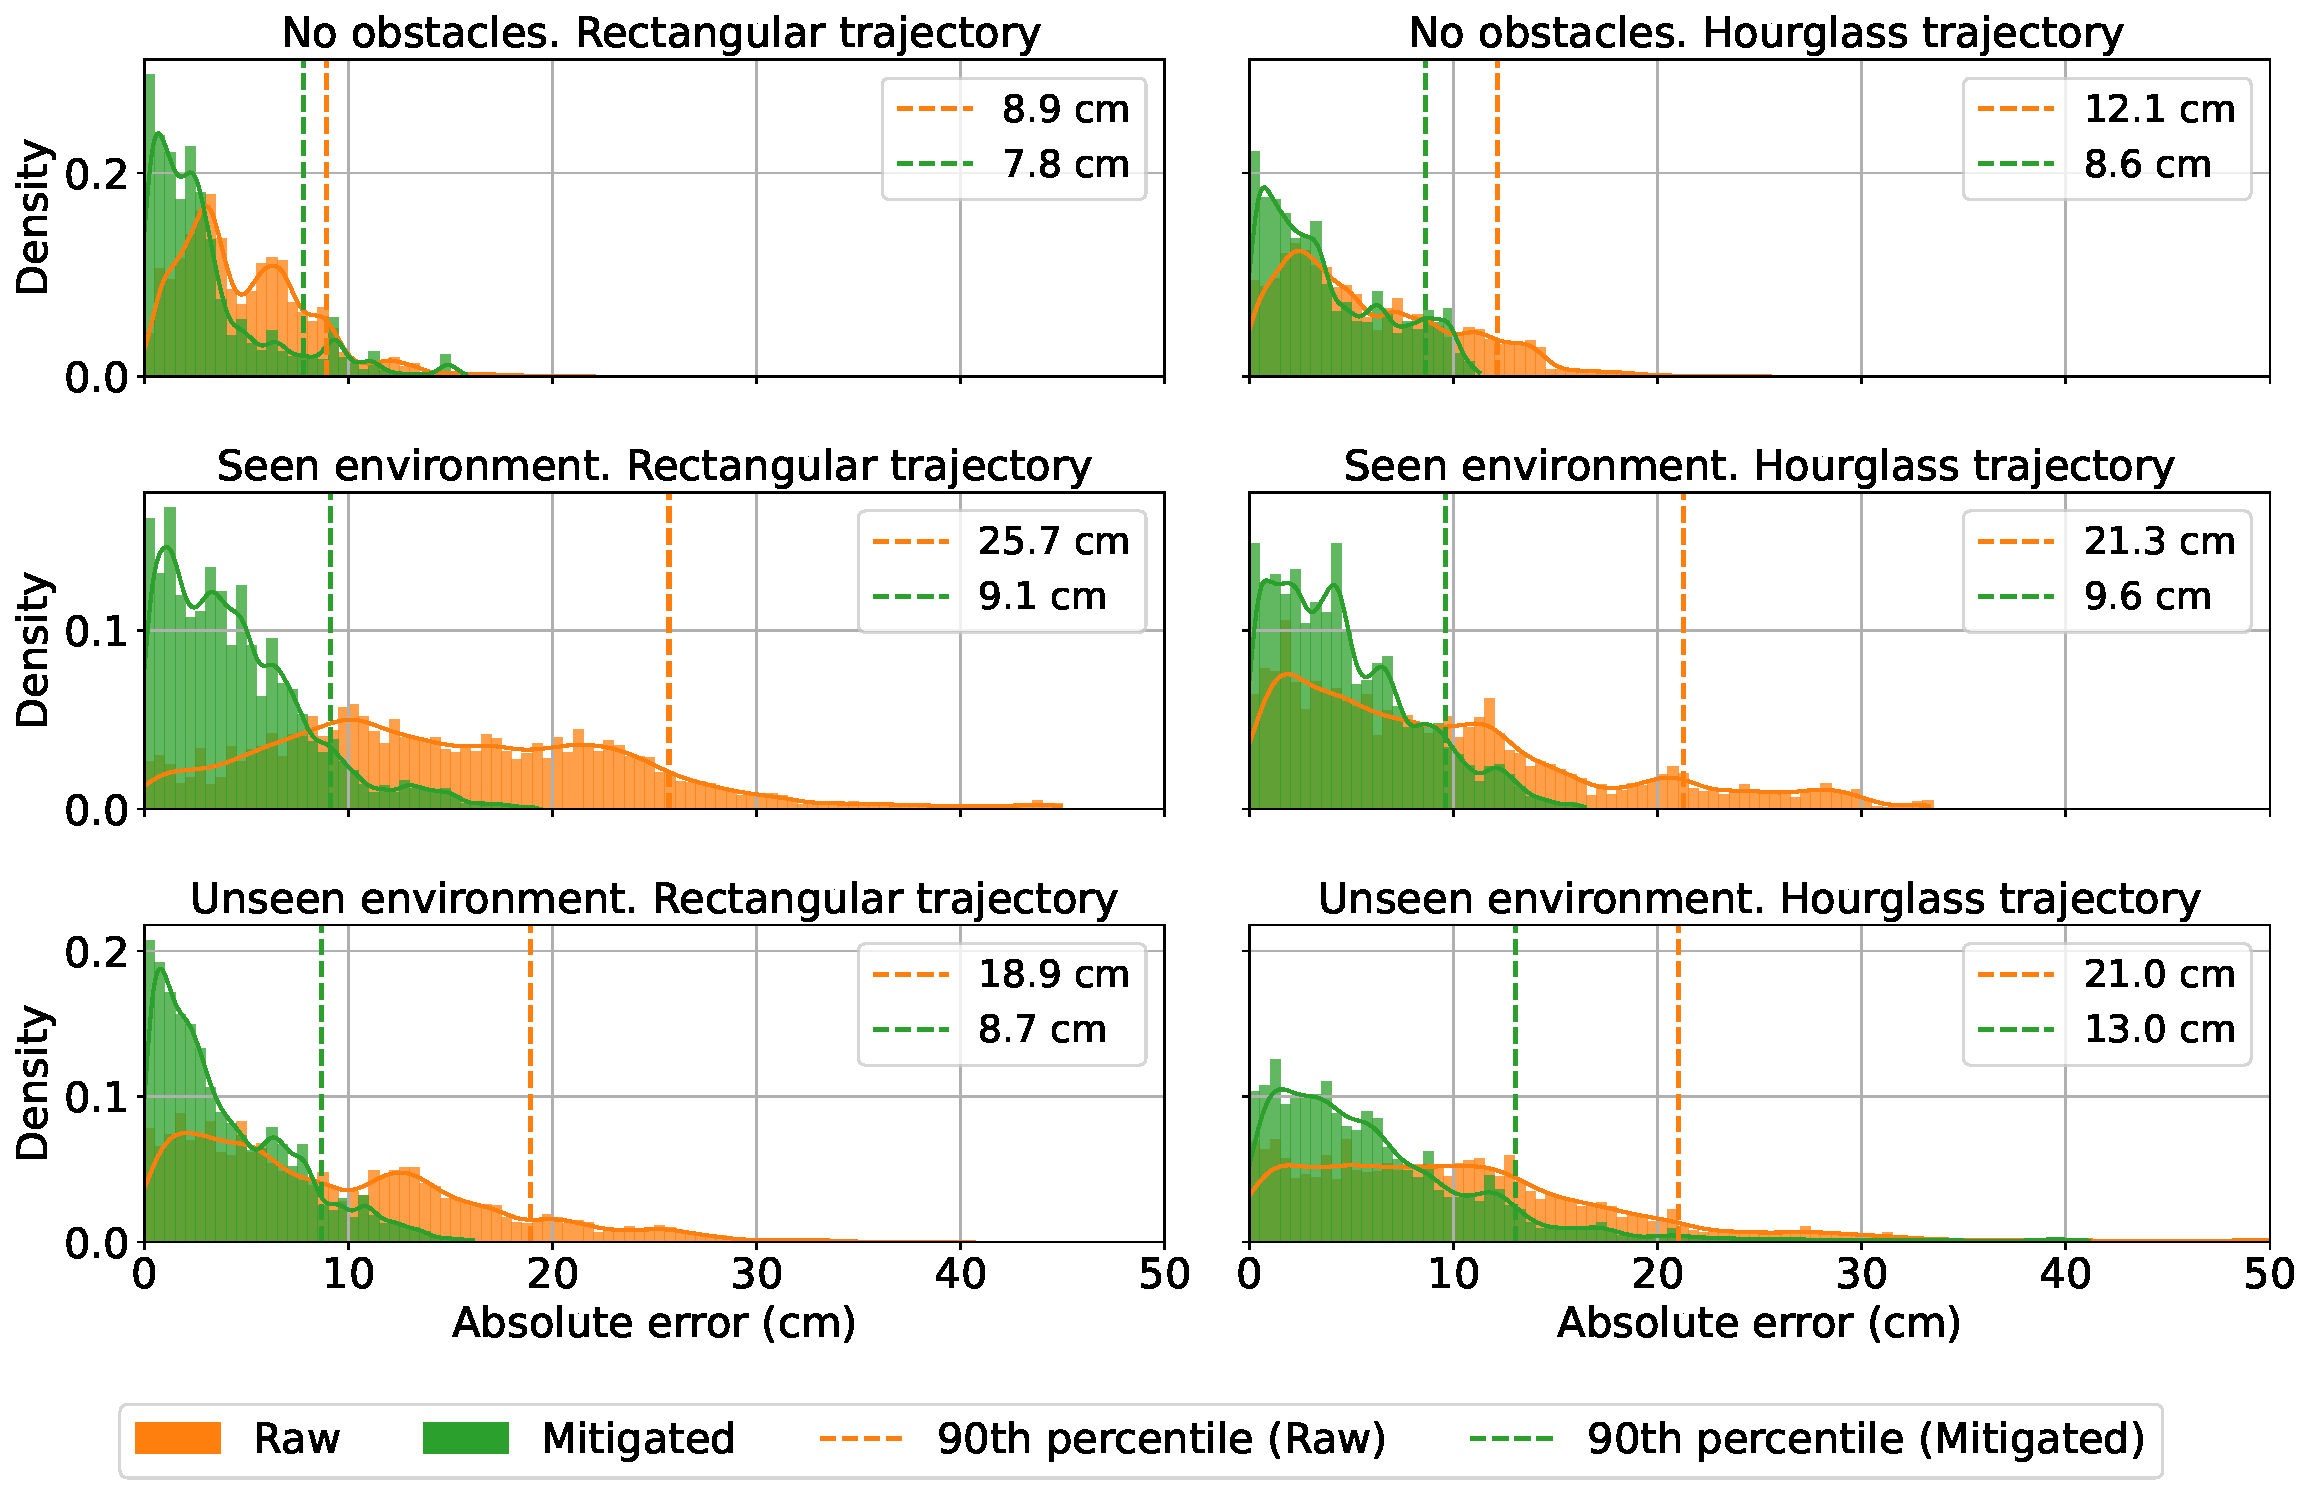
\includegraphics[width=\textwidth]{Figures/experiments_and_results/dtw_errors.pdf}
    \caption[Empirical distributions of localization errors before and after mitigation.]{Empirical distributions of pointwise localization errors before (raw) and after mitigation (mitigated), computed across all experimental repetitions.}
    \label{fig:dtw_errors}
\end{figure}

\autoref{fig:dtw_errors} presents the empirical distributions of pointwise localization errors across all experimental conditions, stratified by environment and trajectory. These are complemented by the corresponding MAE statistics shown in \autoref{fig:dtw_errors_mae_box}, and detailed in \autoref{tab:mae-improvement}, which reports the median MAE before and after error mitigation, along with relative improvements.

Across all evaluated conditions, the error mitigation module consistently yields significant performance gains. As seen in \autoref{fig:dtw_errors}, the application of the proposed model results in a pronounced leftward shift in the error density, indicating a general reduction in estimation errors. Additionally, a consistent decrease in residual error dispersion and MAE is observed, as summarized in \autoref{fig:dtw_errors_mae_box}.

\begin{table}[tbh]
\centering
\caption[Median error and relative improvement for each setup.]{Median MAE and relative improvement for each setup. All values are in centimeters. The $\pm$ denotes standard deviation.}
\label{tab:mae-improvement}
\begin{tabular}{llccc}
\toprule
\textbf{Setup} & \textbf{Trajectory} & \multicolumn{2}{c}{\textbf{MAE}} & \textbf{Improvement} \\
\cmidrule(lr){3-4}
 & & \textit{Raw} & \textit{Mitigated} & \\
\midrule
\multirow{2}{*}{No obstacles} 
  & Rectangular &  5.0 $\pm$ 0.3 & 3.1 $\pm$ 0.3 & \textbf{38} $\pm$ 1 \% \\
  & Hourglass   &  5.8 $\pm$ 0.1 & 3.8 $\pm$ 0.2 & \textbf{33} $\pm$ 3 \% \\
\midrule
\multirow{2}{*}{Seen environment} 
  & Rectangular & 15.9 $\pm$ 0.9 & 4.4 $\pm$ 0.1 & \textbf{70} $\pm$ 4 \% \\
  & Hourglass   &  8.6 $\pm$ 0.6 & 4.5 $\pm$ 0.4 & \textbf{47} $\pm$ 6 \% \\
\midrule
\multirow{2}{*}{Unseen environment} 
  & Rectangular &  9.3 $\pm$ 1.7 & 3.8 $\pm$ 0.5 & \textbf{58} $\pm$ 3 \% \\
  & Hourglass   & 11.9 $\pm$ 1.2 & 7.0 $\pm$ 1.2 & \textbf{41} $\pm$ 3 \% \\
\bottomrule
\end{tabular}
\end{table}

\begin{figure}[tbh]
    \centering
    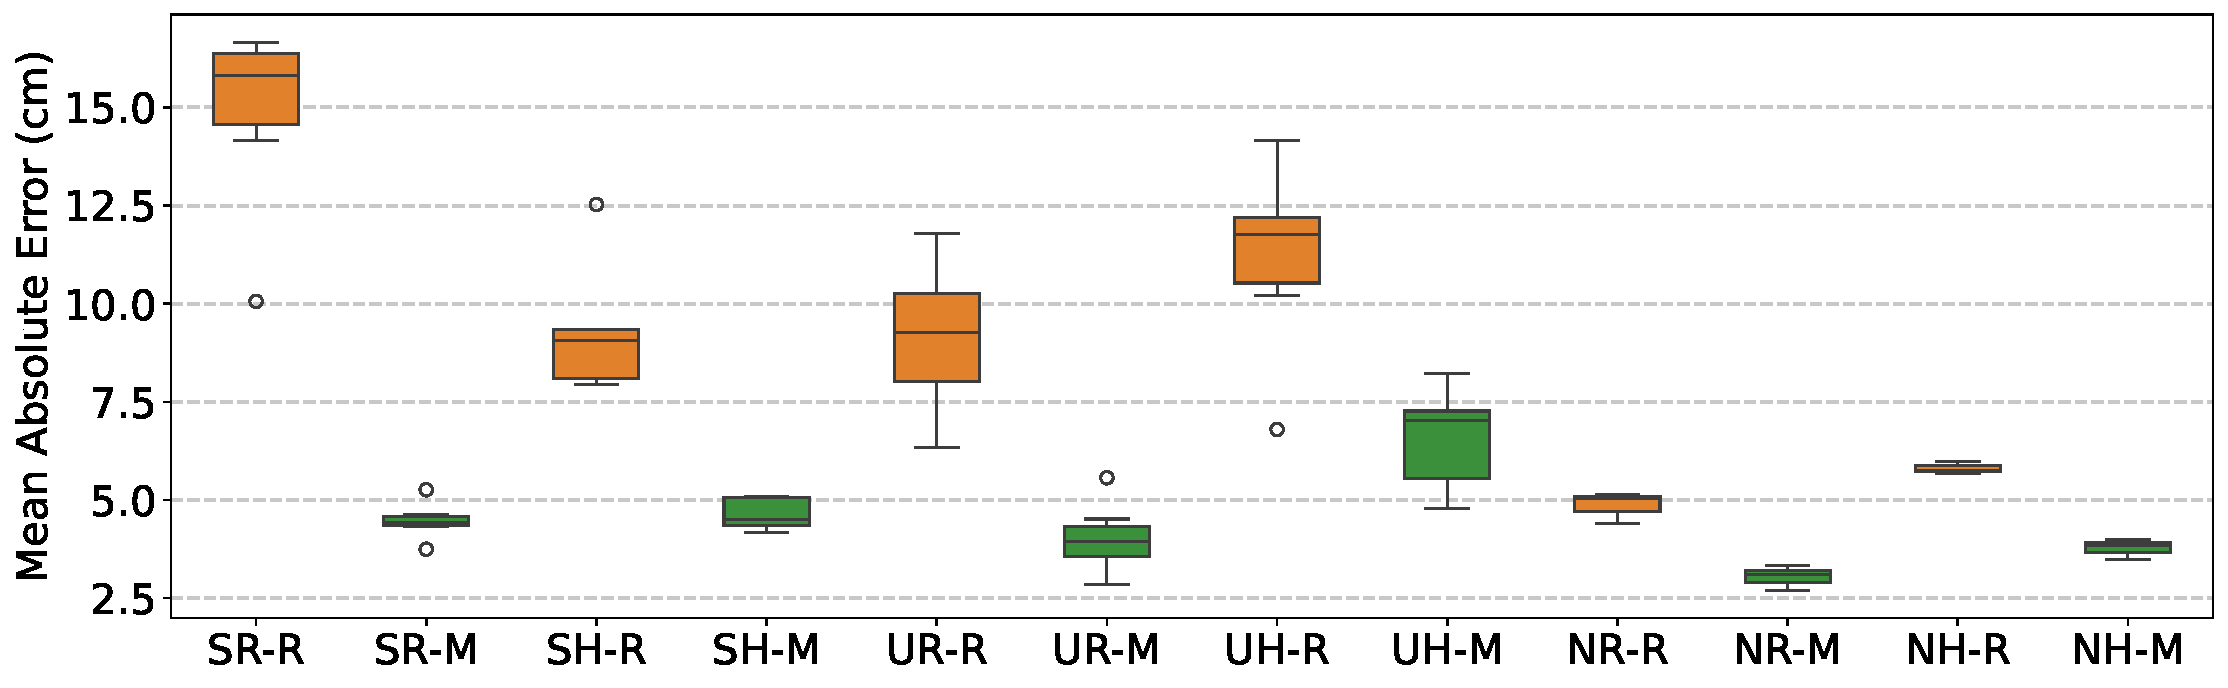
\includegraphics[width=\textwidth]{Figures/experiments_and_results/dtw_errors_mae_box.pdf}
    \caption[Statistics of mean absolute error across all evaluation setups.]{Statistics of MAE across evaluation setups. X-axis labels denote the environment (N -- no obstacles, S -- seen, U -- unseen), trajectory (R -- rectangular, H -- hourglass), and method (R -- raw (orange), M -- mitigated (green)). Individual dots indicate outliers. Refer to \autoref{fig:ranging_accuracy} for details on the interpretation of box plot elements.}
    \label{fig:dtw_errors_mae_box}
\end{figure}

In the LoS configuration, where the initial localization errors are already relatively small (median MAE ranging from 5.0 to 5.8 \si{\centi\meter}), the model achieves a relative improvement of 33-38 \si{\percent}, reducing the residual error to 3.1-3.8 \si{\centi\meter}. Notably, that these values closely approach the fundamental accuracy limits of the ranging subsystem, as established in prior evaluation. We believe, that observed correction likely reflects the model’s capacity to account for systematic errors, such as those arising from antenna radiation patterns, as earlier hypothesized.

The most substantial improvements are observed in the seen NLoS configuration. Here, the mitigation effectively suppresses heavy error tails and significantly reduces the 90th percentile error by up to \SI{16}{\centi\metre}. In particular, the rectangular trajectory exhibits a reduction in median MAE from \SI{15.9}{\centi\metre} to \SI{4.4}{\centi\metre}, corresponding to a \SI{70}{\percent} improvement. For the hourglass trajectory, the error decreases from \SI{8.6}{\centi\metre} to \SI{4.5}{\centi\metre} (\SI{47}{\percent} improvement). While the overall dispersion is also reduced, the gains are smaller than for the rectangular path. This discrepancy is likely related to the increased complexity of the hourglass-shaped trajectory, introduced by sharper turns and a higher likelihood of self-shadowing from the moving subject in this configuration.

In the unseen environment, performance degrades slightly, as expected. Nevertheless, the model continues to achieve meaningful improvements across all runs. The 90th percentile error is reduced by up to \SI{10}{\centi\metre}, and the MAE remains significantly improved. The rectangular trajectory again yields better results, with the MAE decreasing from \SI{9.3}{\centi\metre} to \SI{3.8}{\centi\metre} (\SI{58}{\percent} improvement). For the hourglass trajectory, the error is reduced from \SI{11.9}{\centi\metre} to \SI{7.0}{\centi\metre}, corresponding to a \SI{41}{\percent} improvement. Notably, for the latter configuration, we do not observe a reduction in error dispersion, suggesting that residual errors in retain greater variability. Nonetheless, the overall error remains significantly reduced, and the results indicate that the model generalizes well, achieving \SI{50}{\percent} MAE reduction on average in the unseen setting.

\subsubsection{Qualitative results}

\begin{figure}[tbh]
    \centering
    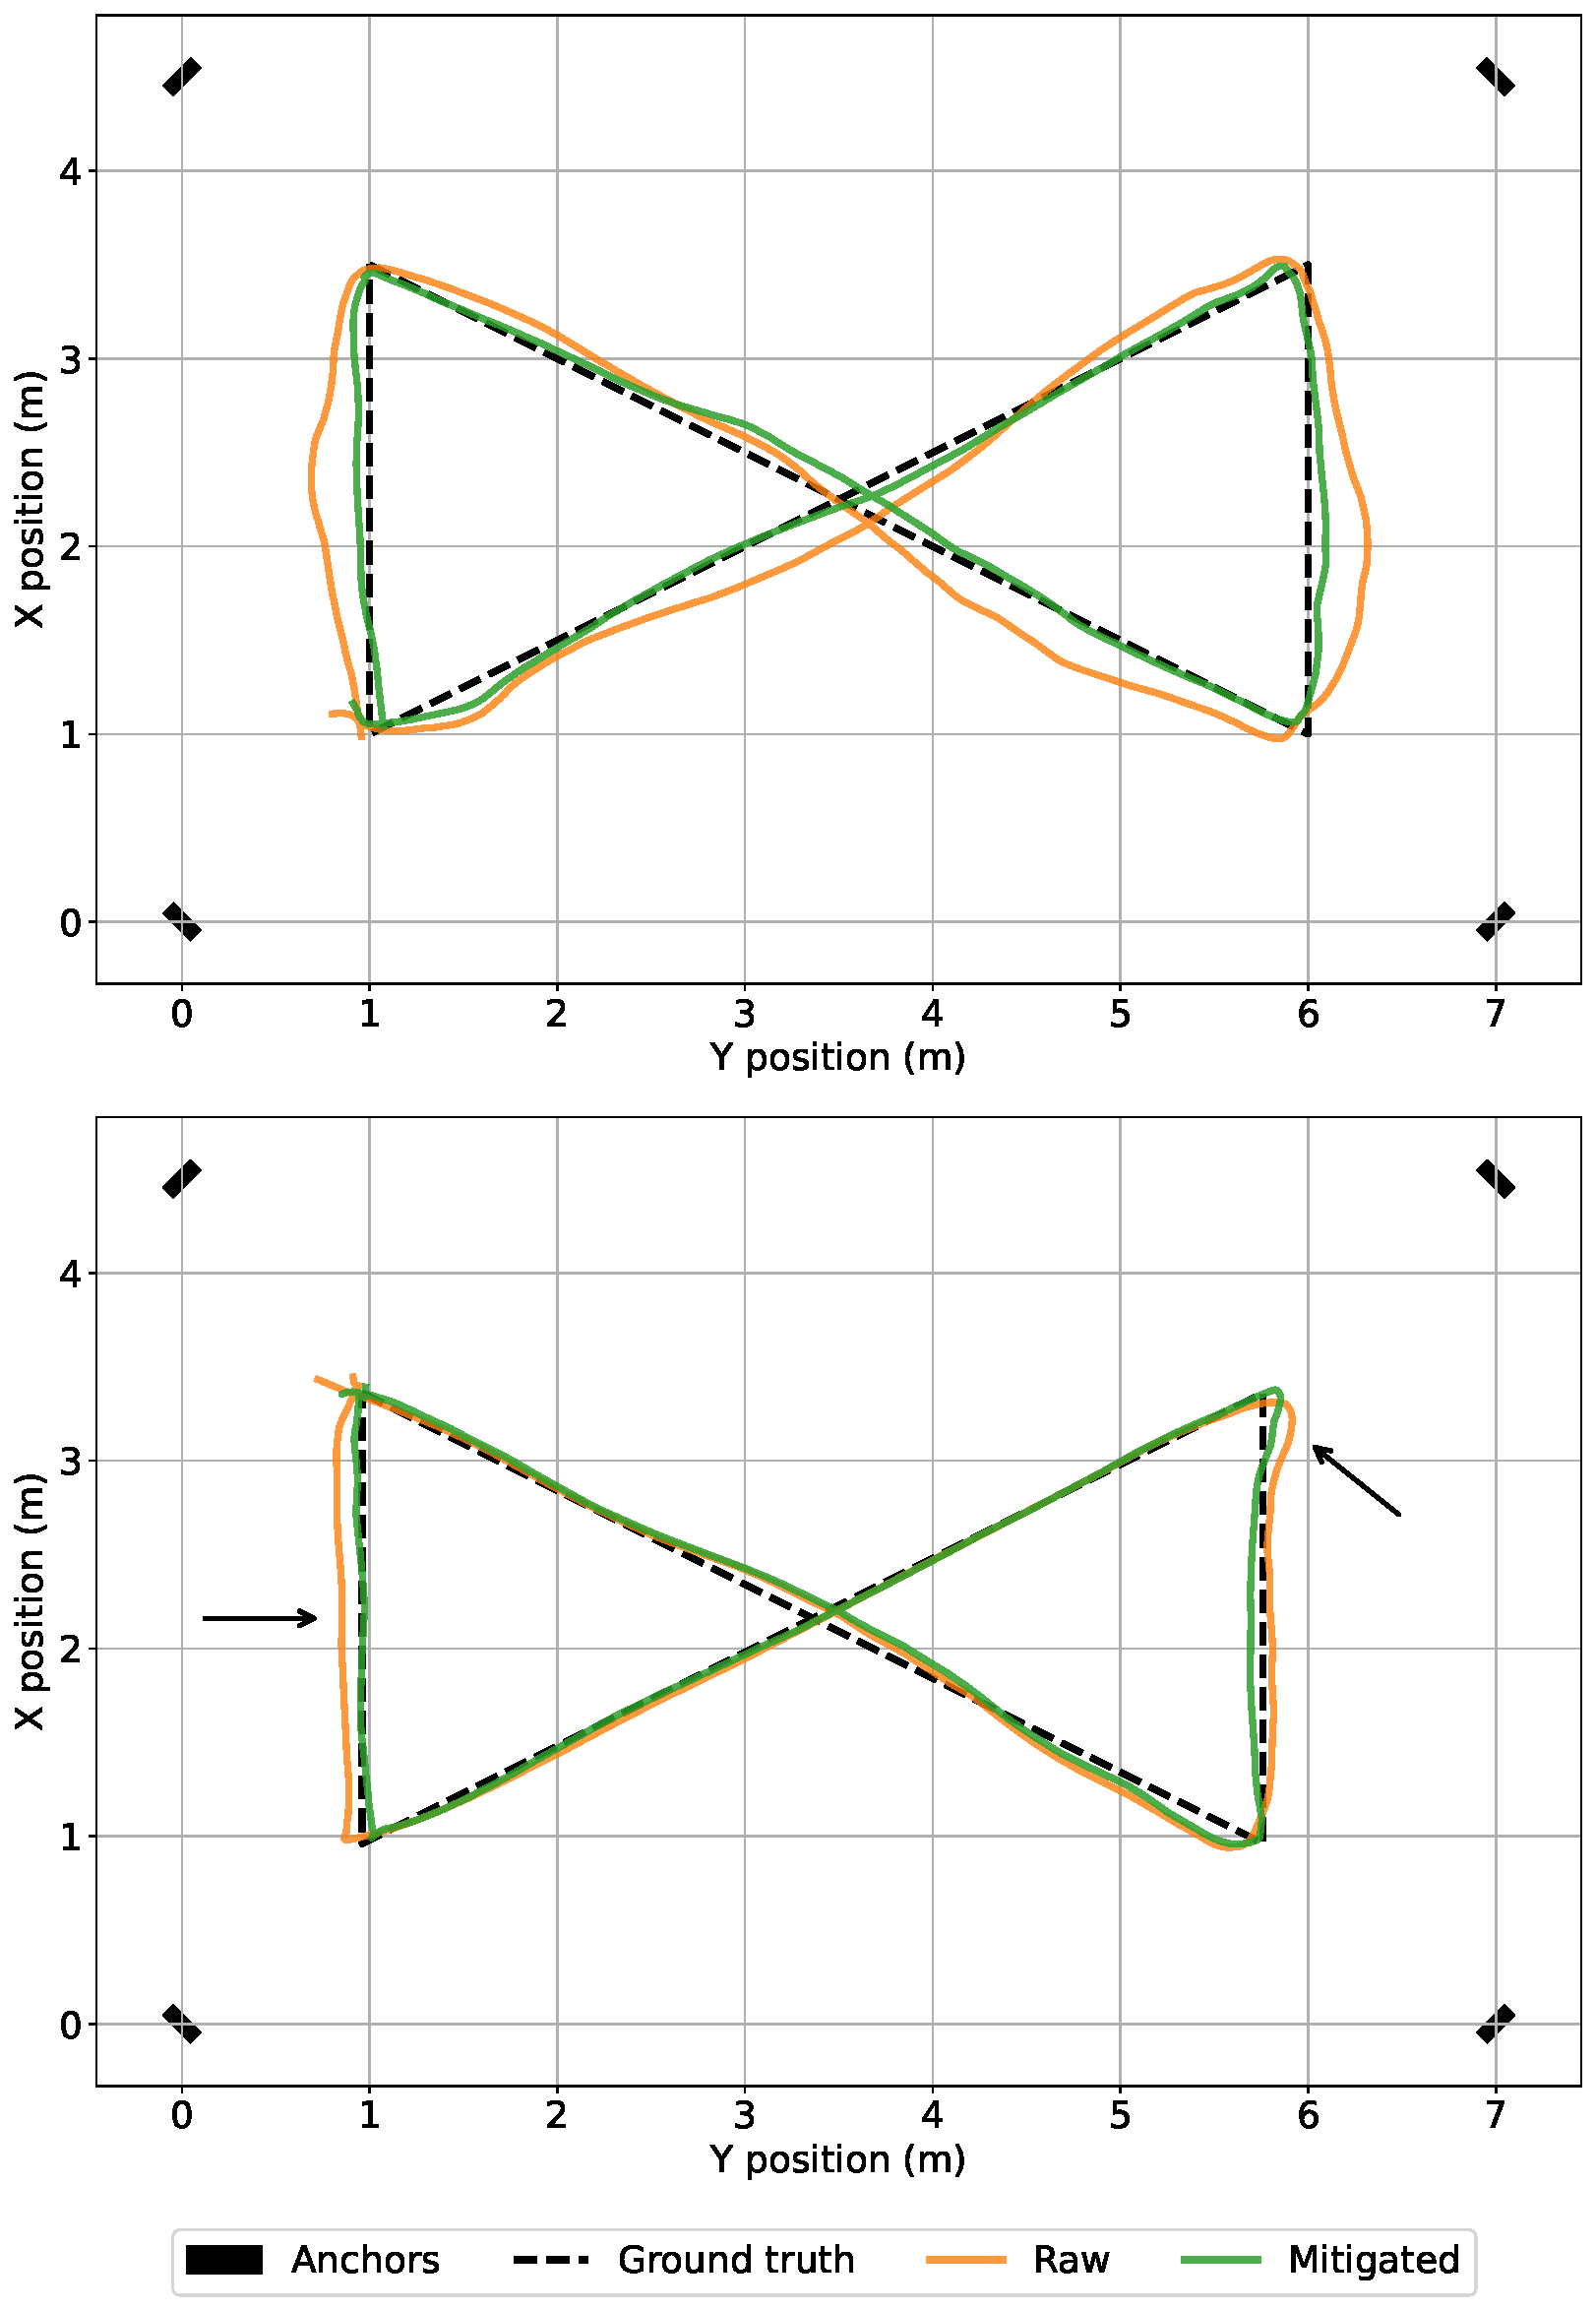
\includegraphics[width=0.85\textwidth]{Figures/experiments_and_results/hourglass_trajectory.pdf}
    \caption{Trajectory reconstruction results for the hourglass trajectory in both LoS (top) and unseen NLoS (bottom) scenarios. Arrows annotate key regions of improvement.}
    \label{fig:trajectories_hourglass}
\end{figure}

\begin{figure}[tbh]
    \centering
    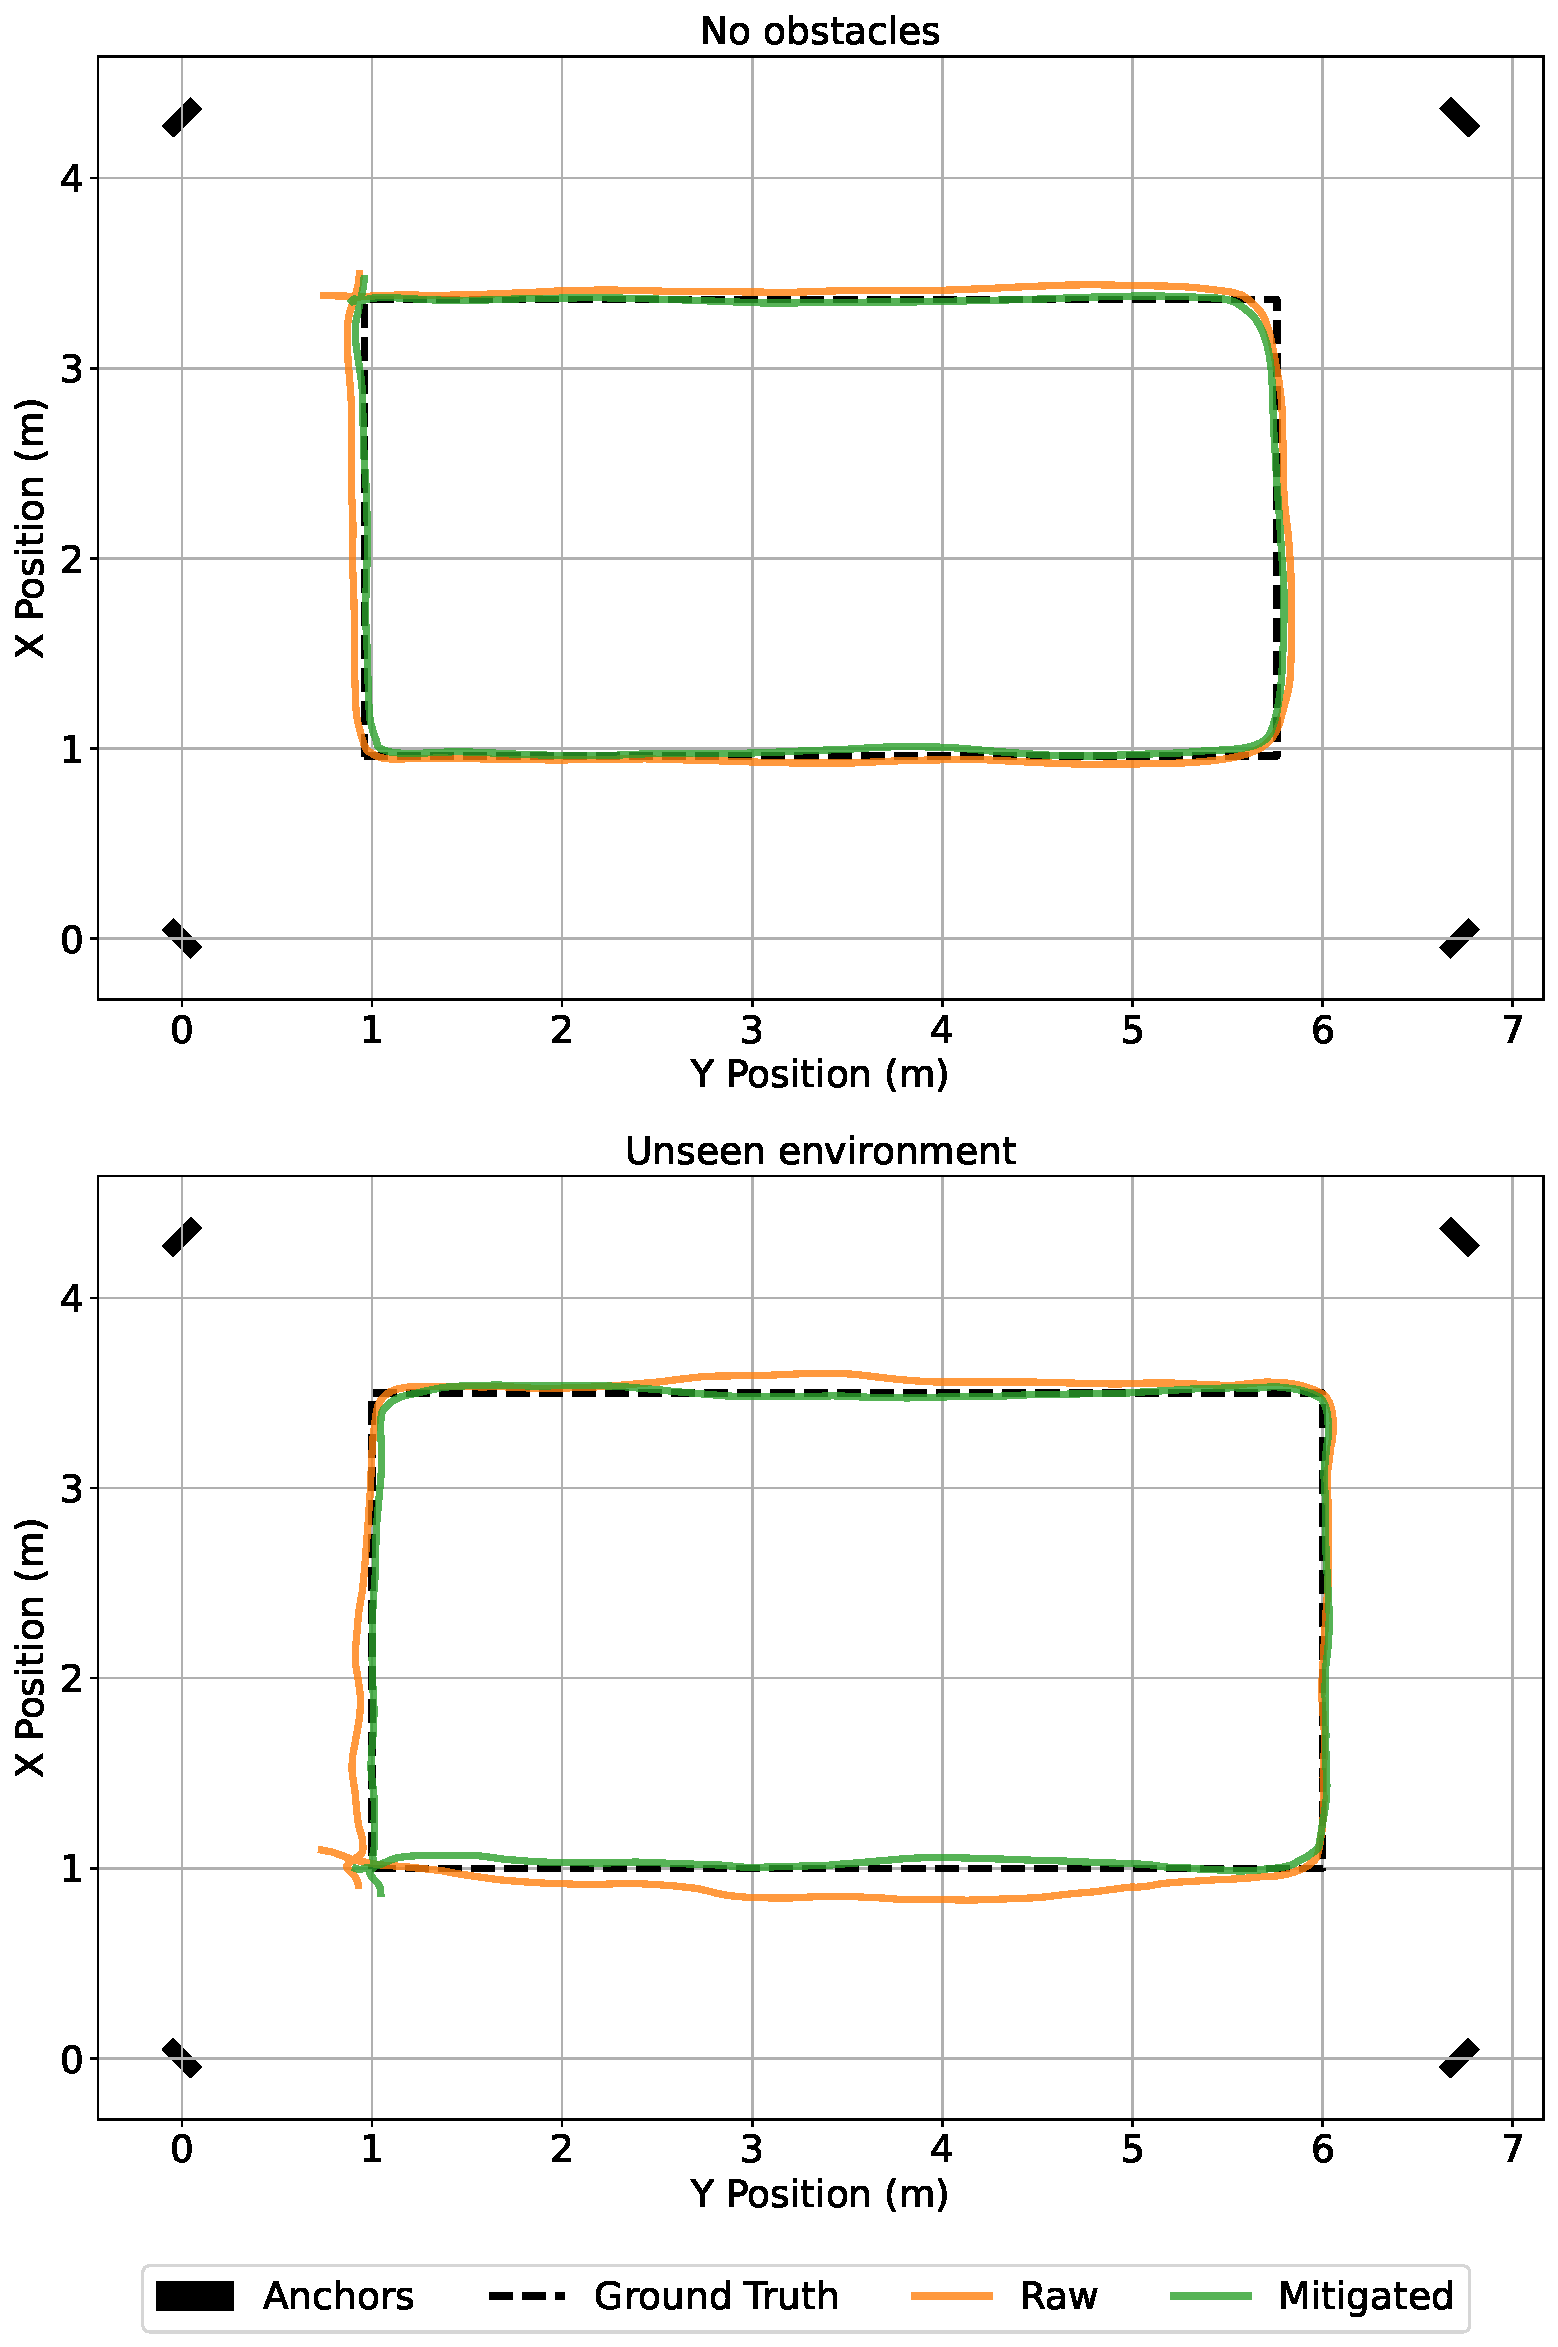
\includegraphics[width=0.85\textwidth]{Figures/experiments_and_results/rect_trajectory.pdf}
    \caption{Trajectory reconstruction results for the rectangular trajectory in both LoS (top) and unseen NLoS (bottom) scenarios.}
    \label{fig:trajectories_rectangle}
\end{figure}

% To illustrate typical performance visually, we present qualitative comparisons of raw versus mitigated estimates against ground truth, for the hourglass and rectangular trajectories in \autoref{fig:trajectories_hourglass}, and \autoref{fig:trajectories_rectangle}, respectively. 

To complement the quantitative results, we present visual examples of typical trajectory reconstruction performance for LoS and unseen NLoS conditions. \autoref{fig:trajectories_hourglass} and \autoref{fig:trajectories_rectangle} illustrate qualitative comparisons between raw and mitigated trajectories versus the ground truth, for the hourglass-shaped and rectangular paths, respectively.

In both cases, the mitigated trajectory has improved geometric alignment with the ground-truth. Even in the LoS case, where original trajectory does not exhibit significant deviations from the ground truth, the mitigated path more closely follows the true one, particularly around trajectory sides. In the unseen environment, where both the room geometry and structural properties, such as building materials and internal layout, differ from the training setup, uncorrected trajectories exhibit significant deviations along all path. The mitigated outputs, however, show considerably reduced overshoot, indicating that the proposed model effectively compensates for NLoS-induced bias despite the domain shift, demonstrating strong generalization.
